\section{Auswertung}
\label{sec:Auswertung}
\subsection{Fehlerrechnung}
Die Fehlerfortpflanzung einer Abgeleiteten Größe $f(x_1,x_2,\ldots,x_n)$ mit den Messunsicherheiten $\symup{\Delta}x_1,\symup{\Delta}x_2,\ldots,\symup{\Delta}x_n$ wird nach Gauß
\begin{equation*}
  \symup{\Delta}f = \sqrt{\left(\frac{\partial f}{\partial x_1}\symup{\Delta}x_1\right)^2 + \left(\frac{\partial f}{\partial x_2}\symup{\Delta}x_2\right)^2 + \ldots + \left(\frac{\partial f}{\partial x_n}\symup{\Delta}x_n\right)^2}
\end{equation*}
berechnet.
\subsection{Messung 30-1000 milli Bar}
\label{subsec:M30-1000}
Der Logarithmus der genommenen Messwerte im Druckbereich von $30-1000\unit{\milli\bar}$ aus \autoref{tab:Tabelle1} werden zunächst in \autoref{fig:M30-1000}
gegen die reziproke Temperatur aufgetragen und eine Ausgleichsrechnung nach \eqref{eqn:ClausInt} mit
\begin{equation}
  \ln\left(p\right) = \frac{m}{T} + b_1
\end{equation}
durchgeführt, wobei
\begin{equation*}
  m = -\frac{L}{R}
\end{equation*}
ist und $R =\SI{8,314}{\joule\per\kelvin\per\mol}$ die allgemeine Gaskonstante \cite{Gerth}.
\begin{table}
  \centering
  \caption{Daten der Messreihe zwischen $30-1000\unit{\milli\bar}$.}
  \begin{tabular}{cc}
    \toprule
    {$T \mathbin{/} \unit{\celsius}$} &
    {$p \mathbin{/} \unit{\milli\bar}$} \\
    \midrule
      22 &  38 \\
      24 &  43 \\
      26 &  47 \\
      28 &  51 \\
      30 &  56 \\
      32 &  60 \\
      34 &  65 \\
      36 &  69 \\
      38 &  75 \\
      40 &  80 \\
      42 &  88 \\
      44 &  95 \\
      46 & 106 \\
      48 & 118 \\
      50 & 131 \\
      52 & 151 \\
      54 & 160 \\
      56 & 176 \\
      58 & 194 \\
      60 & 210 \\
      62 & 232 \\
      64 & 250 \\
      66 & 273 \\
      68 & 293 \\
      70 & 326 \\
      72 & 355 \\
      74 & 385 \\
      76 & 416 \\
      78 & 446 \\
      80 & 488 \\
      82 & 529 \\
      84 & 573 \\
      86 & 614 \\
      88 & 660 \\
      90 & 707 \\
      92 & 759 \\
      94 & 819 \\
      96 & 880 \\
      98 & 938 \\
      100 & 1010 \\
    \bottomrule
  \end{tabular}
  \label{tab:Tabelle1}
\end{table}
\begin{figure}[H]
  \centering
  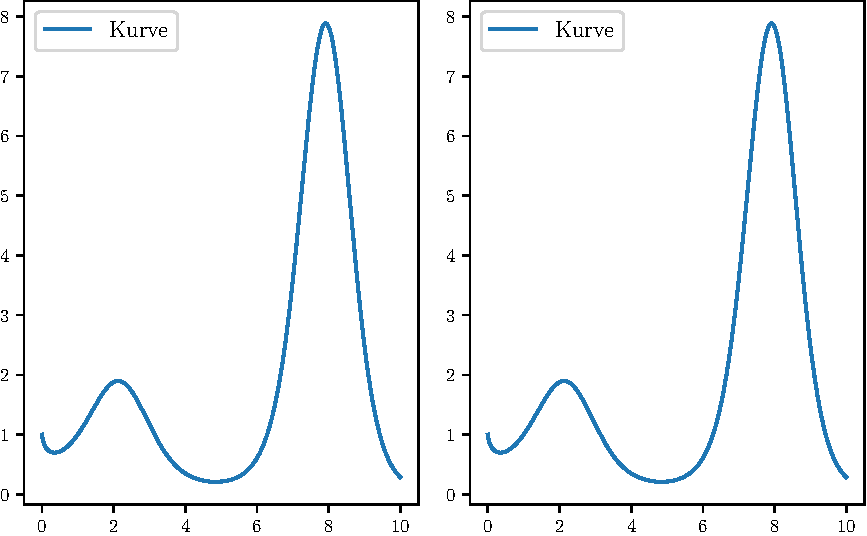
\includegraphics{plot.pdf}
  \caption{Der $\ln\left(p\right)$ gegen die reziproke Temperatur $\frac{1}{T}$ aufgetragen.}
  \label{fig:M30-1000}
\end{figure}
\noindent Die Parameter ergeben sich zu
\begin{align*}
  m &= (-4725.5611\pm 36.9351)\unit{\kelvin}\\
  b_1 &= (12.6472\pm 0.1113),
\end{align*}
woraus für den gemittelten Wert von $L$
\begin{equation*}
  L = -mR = (39290,2052\pm 307,0932)\unit{\joule\per\mol}
\end{equation*}
folgt. Damit soll nun die Größe $L_i = L - L_a$ pro Molekül bestimmt werden, wobei die äußere Verdampfungswärme $L_a$ mithilfe der allgemeine Gasgleichung bei $T = \SI{373}{\kelvin}$ zu
\begin{equation*}
  L_a = RT = (3101,122)\unit{\joule\per\mol}
\end{equation*}
bestimmt wurde. Damit folgt für $L_i$
\begin{equation*}
  L_i = (36189,0832\pm 307,0932)\unit{joule\per\mol}.
\end{equation*}
Die Energie pro Molekül $\frac{L_i}{N_a}$ mit der Avogadrakonstante $N_a = 6,0221\cdot 10^{23}\symup{mol}^{-1}$\cite{Gerth} ergibt sich zu
\begin{equation*}
  \frac{L_i}{N_a} = (0,3751\pm 0.0032)\unit{\electronvolt}.
\end{equation*}
%L = - m * R = 39290,2052 +- 307,0932 J/mol
%R*T = 8,314J/(K*mol)*373K = 3101,122J/mol = L_a
%L_i = L - L_a = 36189,0832 +- 307,0932 J/mol
%pro Molekül: L_i/N_a = 36189,0832 +- 307,0932J/mol / 6,0221*10^23 mol^-1 = 6.0094*10^-20 +- 5.0994*10^-22J
%in eV: 0.3751 +- 0.0032eV
\subsection{Messung 1-15 Bar}
Die Clausius-Calpeyronsche Gleichung \eqref{eqn:Claus} nach L aufgelöst ergibt
\begin{equation}
  \label{eqn:Clausius}
  L = T\left(V_D - V_F\right)\frac{dp}{dT}.
\end{equation}
Um den darin enthaltenen Differentialquotient zu bestimmen, wird $p(T)$ mit dem Polynom
\begin{equation}
  \label{eqn:ApproxP}
  p\left(T\right) = a_1T^3 + b_2T^2 + cT + d
\end{equation}
3.Grades genähert. Mit den Messwerten aus \autoref{tab:Tabelle2} ergibt sich die in \autoref{fig:M1-15} dargestellte Ausgleichsgerade
und die Parameter aus \eqref{eqn:ApproxP} ergeben sich zu
\begin{align*}
  a_1 &= (9.5245\pm 5.5237)\cdot 10^{-1}\unit{\pascal\per\cubic\kelvin} \\
  b_2 &= (-1.0592\pm 0.7025)\cdot 10^3\unit{\pascal\per\kelvin\squared} \\
  c &= (3.9451\pm 2.9721)\cdot 10^5\unit{\pascal\per\kelvin} \\
  d &= (-4.9683\pm 4,1826)\cdot 10^7\unit{\pascal}.
\end{align*}
Leitet man nun \eqref{eqn:ApproxP} nach $T$ ab erhält man den Ausdruck
\begin{equation}
  \frac{dp}{dT} = 3a_1T^2 + 2b_2T + c
\end{equation}
für den Differentialquotienten.\\
Es ist weiterhin $V_F$ gegenüber $V_D$ vernachlässigbar und für $V_D$ gilt die Näherung
\begin{equation}
  \left(p + \frac{a_2}{V^2}\right)V = RT
\end{equation}
mit $a_2 = \SI{0,9}{\joule\cubic\meter\per\mol\squared}$. Wird diese nach $V_D$ aufgelöst ergibt sich
\begin{equation}
  V_{D\pm} = \frac{RT}{2p}\pm\sqrt{\frac{R^2T^2}{4p^2}-\frac{a_2}{p}}.
\end{equation}
In \eqref{eqn:Clausius} eingesetzt folgt für $L$
\begin{equation}
  \label{eqn:LT}
  L_{\pm} = T\left(\frac{RT}{2p}\pm\sqrt{\frac{R^2T^2}{4p^2}-\frac{a_2}{p}}\right)\frac{dp}{dT}.
\end{equation}
$L$ ist für die gemessenen Werte aus \autoref{tab:Tabelle2} in \autoref{fig:LAdd}(Addition der Wurzel) und \autoref{fig:LSub}(Subtraktion der Wurzel) dargestellt.
%Params[ 9.62448345e-06 -1.05917151e-02  3.94505696e+00 -4.96834748e+02] Fehler[5.52371428e-06 7.02493794e-03 2.97205249e+00 4.18264509e+02]
\begin{table}[H]
  \centering
  \caption{Daten der Messreihe zwischen $1-15\unit{\bar}$.}
  \begin{tabular}{cc}
    \toprule
    {$p \mathbin{/} \unit{\bar}$} &
    {$T \mathbin{/} \unit{\celsius}$} \\
    \midrule
      1 & 108 \\
      2 & 120 \\
      3 & 134 \\
      4 & 140 \\
      5 & 148 \\
      6 & 156 \\
      7 & 160 \\
      8 & 166 \\
      9 & 170 \\
      10 & 174 \\
      11 & 177 \\
      12 & 182 \\
      13 & 187 \\
      14 & 189 \\
      15 & 190 \\
    \bottomrule
  \end{tabular}
  \label{tab:Tabelle2}
\end{table}
\begin{figure}[H]
  \centering
  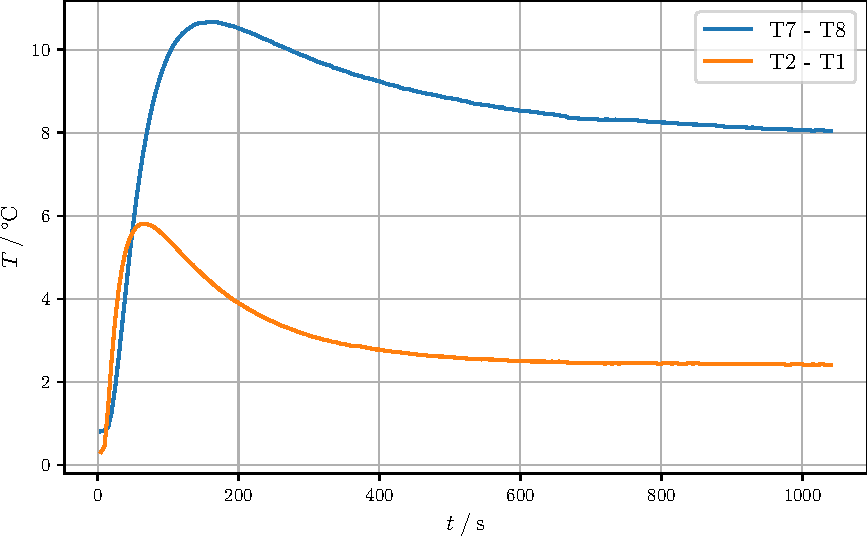
\includegraphics{plot2.pdf}
  \caption{Der Druck $p$ gegen die Temperatur $T$ aufgetragen.}
  \label{fig:M1-15}
\end{figure}
\begin{figure}[H]
  \centering
  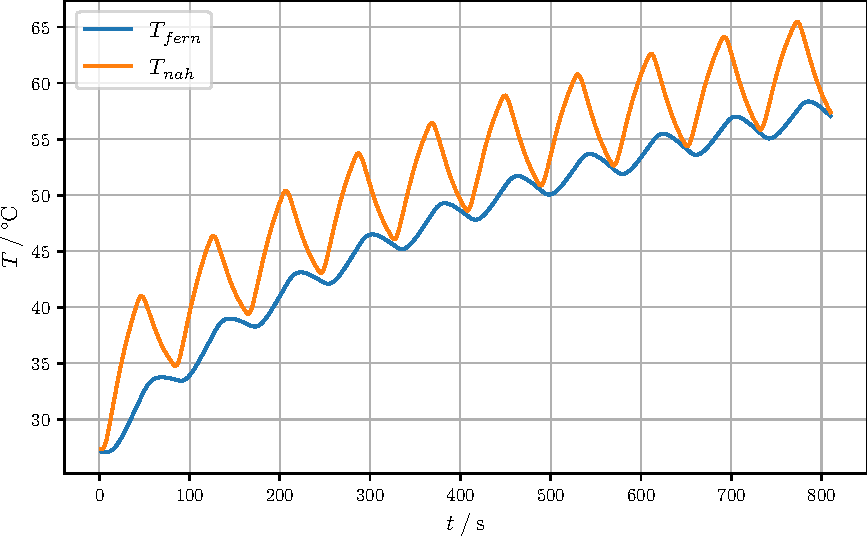
\includegraphics{plot3.pdf}
  \caption{$L$ gegen die Temperatur $T$ aufgetragen bei Addition der Wurzel.}
  \label{fig:LAdd}
\end{figure}
\begin{figure}[H]
  \centering
  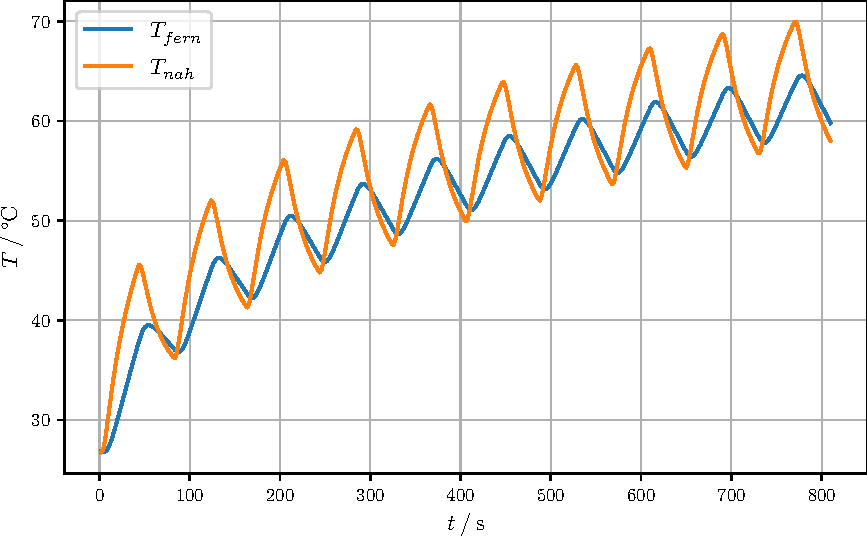
\includegraphics{plot4.pdf}
  \caption{$L$ gegen die Temperatur $T$ aufgetragen bei Subtraktion der Wurzel.}
  \label{fig:LSub}
\end{figure}
